\section{Introduction}
\columnbreak
\begin{figure}[t]
    \centering
    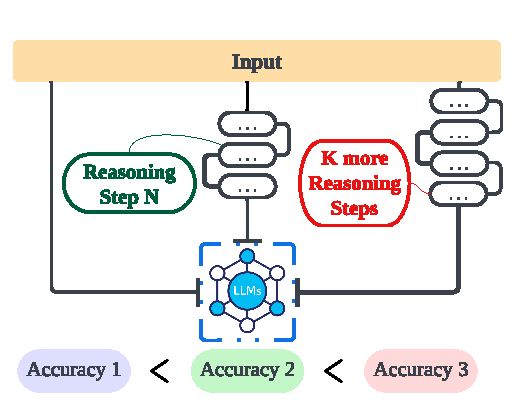
\includegraphics[width=0.9\columnwidth]{add.pdf}
    \caption{From left to right: zero-shot CoT, few-shot CoT, and few-shot CoT with more reasoning steps. For few-shot COT, there is a direct linear correlation between step count and accuracy.}
    \label{fig:steps-connection-with-accuracy}
\end{figure}

Today, the advent of large language models (LLMs) and their advanced prompting strategies has marked a significant progression, especially in classical NLP tasks \cite{kojima2023large,wei2022chain,shao2023synthetic,lyu2023faithful, jin2024exploring}. A key innovation among these is the Chain of Thought (CoT) prompting technique \cite{kojima2023large,wang2023selfconsistency,zhang2022automatic}, known for its efficacy in multi-step problem solving. This technique, reflecting human sequential reasoning, has shown remarkable effectiveness in various challenges, including cross-domain, length-generalization, and cross-lingual tasks. The CoT approach, with its logical, step-by-step methodology, offers crucial interpretability in complex problem-solving scenarios. Interestingly, \citeauthor{wang2023selfconsistency} found that even incorrect but coherent rationales can improve reasoning performance, highlighting the value of logical continuity \cite{wang2023selfconsistency}. Building on this, \citeauthor{fu2023complexitybased} introduced complexity-based prompting, significantly improving accuracy and setting new benchmarks \cite{fu2023complexitybased}. This research further explores the relationship between the length of reasoning steps and the accuracy of conclusions, deepening our understanding of effective problem-solving in NLP.

Despite its promising results, the research community has yet to reach a consensus on the precise mechanics of how and why CoT and its variations function effectively. This knowledge gap means that enhancing CoT performance is still a field of exploration, largely reliant on trial-and-error approaches. There still lack established systematic methodologies for improving CoT's effectiveness, leaving researchers to rely on conjecture and experimentation. This situation underscores a significant opportunity in the field: to develop a deeper, more structured understanding of CoT's inner workings. Such advancement would not only demystify the current process, but also pave the way for more reliable and efficient applications of this technique in various complex NLP tasks.

In this study, we aim to investigate the hypothesis that the reasoning steps are the most crucial element in the effectiveness of CoT prompts. This hypothesis stems from the observation that reasoning steps are a common element in both zero-shot and few-shot CoT approaches. We conduct experiments to investigate this by maintaining strict control over variables. Particularly, when incorporating new reasoning steps, we ensured that no additional knowledge was introduced. For the zero-shot experiments, we tweaked the initial prompt from ``let's think step by step'' to ``let's think step by step, you must think more steps''. Then for few-shot setting, we design experiments that expand the rationale reasoning steps within CoT demonstrations, while keeping all other factors constant.
Our first set of experiments evaluated the improvement in zero-shot and few-shot performance using Auto-CoT~\cite{zhang2022automatic} with our strategic intervention. Subsequently, we assessed the accuracy of different methods across varying step lengths. We then extended our investigation to compare the effectiveness of our strategy on different LLMs such as GPT-3.5 and GPT-4. Our findings revealed a significant correlation between the length of the reasoning chain and the capabilities of LLMs, within certain limits. Intriguingly, when we introduced misleading information into the reasoning chain, the performance still showed improvement. This highlighted a pivotal insight: The key factor appears to be the length of the thinking chain rather than its accuracy.
We have the following key findings, which we hope can help the community better improve CoT performance.
\begin{itemize}[leftmargin=*]\setlength\itemsep{-0.3em}

\item \emph{For few-shot COT, there is a direct linear correlation between step count and accuracy.} This provides a quantifiable approach for optimizing CoT prompting in complex reasoning. Specifically, lengthening the reasoning steps in prompts considerably enhances LLMs' reasoning abilities across multiple datasets. Alternatively, shortening reasoning steps, even while preserving key information, significantly diminishes the reasoning abilities of models.
%
\item \emph{Even incorrect rationales can yield favorable outcomes if the required length of inference is maintained.} For example, in mathematical problems, errors in intermediate numbers have a minor impact due to their process-oriented nature.

\item \emph{The advantages of increasing reasoning steps are task-dependent}: simpler tasks necessitate fewer steps, whereas more complex tasks gain significantly from longer inference sequences.

\item \emph{Increased reasoning steps in zero-shot CoT can also significantly improve LLM accuracy.} To validate this, we altered the initial prompt from ``Let's think step by step" to ``Let's think step by step, you must think more steps." This modification led to a noticeable enhancement in the reasoning abilities of the LLMs, particularly evident in datasets involving mathematical problems.

\end{itemize}